\normaltrue \difficilefalse \tdifficilefalse
\correctionfalse
%\UPSTIidClasse{11} % 11 sup, 12 spé
%\renewcommand{\UPSTIidClasse}{12}

\exer{Train simple $\star$ \label{C2:06:34}}
\textit{D'après documentation F. Mazet.} \\
\setcounter{question}{0}\UPSTIcompetence[2]{A3-05}
\UPSTIcompetence[2]{C2-06}
\index{Compétence C2-06}
\index{Train d'engrenages simple}
\ifcorrection
\else
\marginnote{\textbf{Pas de corrigé pour cet exercice.}}
\fi

\ifprof
\else
On s'intéresse à la chaîne de transmission de puissance du Control'X dont un modèle est donné dans la figure ci-dessous.

On note : 
\begin{itemize}
\item \textbf{0:} le bâti auquel est encastré une couronne de rayon primitif $R_b$;
\item \textbf{1:} le pignon de sortie du moteur de rayon primitif $R_m$;
\item \textbf{2:} un des 3 satellites du réducteur épicycloïdal de rayon primitif $R_s$;
\item \textbf{3:} le porte-satellite auquel est encastré une poulie de rayon $R_p$;
\item \textbf{5:} le chariot de masse $M$ encastré à la courroie \textbf{4} considérée inextensible. On note $v=\vectv{D}{5}{0}\cdot \vect{y}$;
\item \textbf{3:} le seconde poulie de rayon $R_p$;
\end{itemize}


\begin{center}
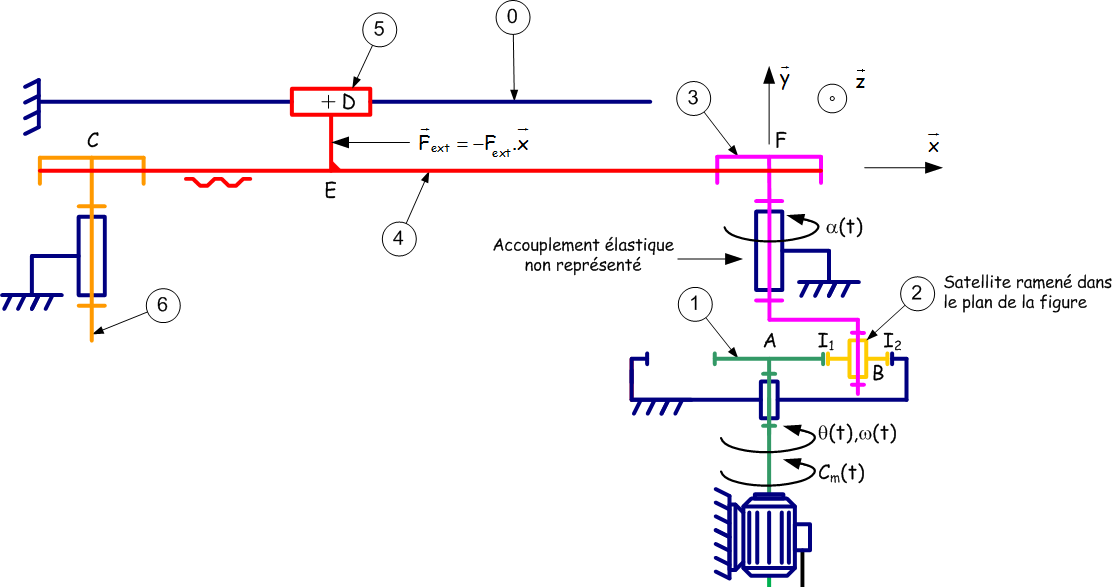
\includegraphics[width=\linewidth]{34_01}
\end{center}
\fi


\question{Déterminer la relation entre $\omega(1/0)$ et $v$.}
\ifprof
\else
\fi



\ifprof
\else
\begin{flushright}
\footnotesize{Corrigé  voir \ref{C2:06:34}.}
\end{flushright}%
\fi